\chapter{Implementierung}
\label{implementierung}
In diesem Kapitel der Arbeit wird auf die Implementierung der Datenbanksystem-spezifischen Adapter von Linkbench eingegangen, die für die Analyse der Performance dieser Systeme notwendig ist. 

Bevor allerdings auf die Implementierung dieser Adapter eingegangen werden kann, muss zuerst auf das Linkbench-Repository eingegangen werden, das für die Implementierung dieser Adapter als Ausgangspunkt dient. Außerdem muss auch ermittelt werden, ob bereits frei verfügbare Db2-Graph- oder Neo4j-spezifische Adapter für Linkbench existieren und ob deren Einsatz bei der Performance-Analyse möglich und sinnvoll ist.

Darüber hinaus wird in diesem Kapitel auch auf kleinere Anpassungen an Linkbench selbst eingegangen. Bei diesen Anpassungen handelt es sich um Änderungen am Benchmark, die außerhalb der Datenbank-spezifischen Adapter durchgeführt werden mussten.

\section{Code-Basis}
\label{implementierung:basis}
Bei den Recherchen nach einer Linkbench-Code-Basis, die als Ausgangspunkt für die Implementierung eigener Datenbank-Adapter oder der Anbindung bereits existierender Datenbank-Adapter an den Benchmark dienen sollte, konnten die beiden folgenden Repositories auf GitHub identifiziert werden:
\begin{itemize}
    \item \texttt{mdcallag/linkbench} \cite{mc_linkbench_github} und 
    \item \texttt{facebookarchive/linkbench} \cite{fb_linkbench_github}.
\end{itemize}
Beide Repositories enthalten dabei eine als Ausgangspunkt nutzbare Implementierung von Linkbench. Schlussendlich fiel die Entscheidung, welche Implementierung als Code-Basis für den Linkbench im Rahmen dieser Arbeit herangezogen werden soll, allerdings auf das \texttt{mdcallag/linkbench}-Repository von \citeAY{mc_linkbench_github}. 

Denn obwohl es sich bei dem \texttt{facebookarchive/linkbench}-Repository um die originale Implementierung des Benchmarks von Facebook handelt, ist die Implementierung von Linkbench im \texttt{mdcallag/linkbench}-Repository weitaus fortgeschrittener als die von Facebook. Dies liegt darin begründet, dass die in \texttt{facebookarchive\allowbreak /linkbench}-Repository befindliche Implementierung von Linkbench nicht mehr aktiv weiter entwickelt wird \cite{fb_linkbench_github}. Der letzte Commit in dem Repository stammt vom 11.12.2015. 

Die Implementierung von Linkbench aus dem \texttt{mdcallag/linkbench}-Repository, ist einen Fork von \texttt{facebookarchive\allowbreak /linkbench}-Repository, der in den letzten Jahren aktiv weiterentwickelt wurde \cite{mc_linkbench_github}. So enthält das \texttt{mdcallag/linkbench}-Repository von \citeAY{mc_linkbench_github} Adapter für die Datenbanksysteme: 
\begin{itemize}
    \item MySQL,
    \item MongoDB und
    \item PostgreSQL.
\end{itemize}
Das \texttt{facebookarchive/\allowbreak linkbench}-Repository hingegen, verfügt ausschließlich über den MySQL-Adapter \cite{mc_linkbench_github}. Darüber hinaus enthält das Repository auch einen generischen SQL-Adapter \cite{mc_linkbench_github}. Dieser kann als Basis für die Implementierung eines Adapters für relationale Datenbanksysteme herangezogen werden \cite{mc_linkbench_github}. Schließlich implementiert er bereits die meisten Operationen für Datenbanksysteme, die JDBC (Java Database Connectivity) als Schnittstelle unterstützen \cite{mc_linkbench_github}. Womöglich könnte der generische SQL-Adapter auch als Basis für die Adapter für Db2 Graph eingesetzt werden, da er bereits einige schreibende Operationen implementiert. Dadurch könnte unter Umständen auch der Aufwand für die Implementierung dieser Adapter gesenkt werden.

Außerdem wurden bei der Implementierung in \texttt{mdcallag/linkbench}-Repository einige Anpassungen vorgenommen, die eine detailliertere Aufschlüsselung der gemessenen Latenzwerte ermöglichen und die Fehlerbehandlung verbessern \cite{mc_linkbench_github}.

\section{Evaluation existierender Adapter}
\label{implementierung:evaluation}
Im Rahmen dieses Unterabschnitts werden bereits existierende Linkbench-Adapter für Db2 Graph und Neo4j aufgeführt und evaluiert. Dabei wird untersucht, ob die Adapter für die Performance-Analyse der Datenbanksysteme dieser Arbeit herangezogen werden können oder ein neuer Adapter implementiert werden muss. 

\subsection{Db2 Graph}
\label{implementierung:evaluation:db2graph}
Bei dem Datenbanksystem Db2 Graph ist bekannt, dass hierfür bereits eine Adapter-Implementierung für Linkbench existieren muss. Schließlich werden im Artikel von \citeAY{sigmod_tian} Db2 Graph Ergebnisse für den Linkbench Benchmark präsentiert. Es gilt allerdings zu beachten, dass der darin eingesetzte Adapter für eine ältere Version von Db2 Graph konzipiert wurde, die unter Umständen nicht mit Db2 Graph Beta 3 und Db2 Graph V11.5.6.0 kompatibel ist. Außerdem wurde der Adapter, wie bereits in \compref{analyse:reproduktion} aufgeführt, nie veröffentlicht. Daher kann der Adapter nicht im Rahmen der Performance-Analyse genutzt werden. Da über diesen Adapter hinaus keine weiteren Adapter-Implementierungen für Db2 Graph bekannt sind, müssen im Rahmen dieser Arbeit eigene Adapter für Db2 Graph Beta 3 und V11.5.6.0 entwickelt werden. 

\subsection{Neo4j}
\label{implementierung:evaluation:neo4j}
Auch ein Adapter für Neo4j muss im Rahmen dieser Arbeit neu implementiert werden. Dies rührt daher, dass der einzig auffindbare, frei verfügbare Neo4j-Adapter von \citeAY{neo_linkbench_github} auf dem technischen Stand von 2013 ist. Infolgedessen ist der Adapter nicht dazu in der Lage, die Fähigkeiten neuer Neo4j-Versionen voll auszuschöpfen. So setzt der Adapter von \citeAY{neo_linkbench_github} zur Interaktion mit Neo4j eine veraltete Java-basierte Traversal-API ein, obwohl inzwischen die Abfragesprache Cypher die bevorzugte Form der Interaktion mit Neo4j ist \cite{gdbms}.

\section{Adapter}
\label{implementierung:adapter}
Da sich die bereits existierenden Adapter für Db2 Graph und Neo4j nicht für den Einsatz im Zuge der Performance-Analyse eignen oder dafür zur Verfügung stehen, müssen im Rahmen dieser Arbeit folgende Adapter implementiert werden:
\begin{itemize}
    \item \texttt{Neo4j}-Adapter für Neo4j,
    \item \texttt{Db2GraphOld}-Adapter für Db2 Graph Beta 3, 
    \item \texttt{Db2Graph}-Adapter für Db2 Graph V11.5.6.0 und
    \item \texttt{Db2}-Adapter.
\end{itemize}
Die Entwicklung von zwei verschiedenen Adaptern für Beta 3 und V11.5.6.0 ist hierbei notwendig, da sich die beiden an einigen Stellen erheblich unterscheiden. So läuft der Verbindungsaufbau und das Session-Management bei beiden Versionen anders ab, wie bereits in \autoref{db2graph:versionen} erläutert. 

Um einen kurzen, anfänglichen Überblick darüber zu bieten, wie die Adapter aufgebaut sind, werden sie in \autoref{fig:adapter_uebersicht} skizziert.

\begin{figure}[!ht]
    \centering
	\usetikzlibrary{arrows, arrows.meta}
	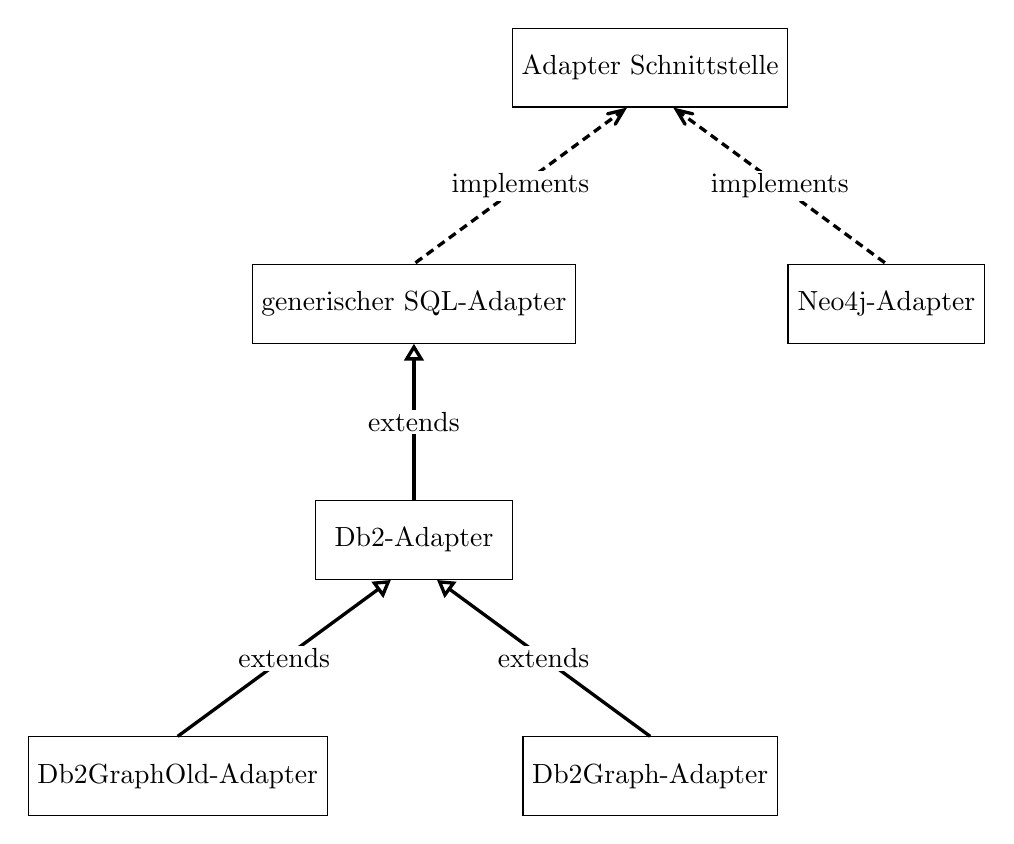
\begin{tikzpicture}[
		nodestyle/.style={draw, minimum height=10mm, minimum width=25mm},
		implements/.style={{angle 45}-, very thick, densely dashed},
		extends/.style={{Triangle[open]}-, very thick},
		linetext/.style={fill=white, inner sep=1pt}
	]
		\node[nodestyle] (interface) at (0, 0) {Adapter Schnittstelle};
		\node[nodestyle] (sql) at (-3, -3) {generischer SQL-Adapter};
		\node[nodestyle] (neo4j) at (3, -3) {Neo4j-Adapter};
		\node[nodestyle] (db2) at (-3, -6) {Db2-Adapter};
		\node[nodestyle] (graphold) at (-6, -9) {Db2GraphOld-Adapter};
		\node[nodestyle] (graph) at (0, -9) {Db2Graph-Adapter};
		
		\draw[implements] (interface.-120) -- node[linetext] {implements} (sql.north);
		\draw[implements] (interface.-60) -- node[linetext] {implements} (neo4j.north);
		\draw[extends] (sql.south) -- node[linetext] {extends} (db2.north);
		\draw[extends] (db2.-120) -- node[linetext] {extends} (graphold.north);
		\draw[extends] (db2.-60) -- node[linetext] {extends} (graph.north);
	\end{tikzpicture}
    \caption{Adapter Übersicht}
    \label{fig:adapter_uebersicht}
\end{figure}


\subsection{Db2-Adapter}
\label{implementierung:adapter:db2}
Bei dem Db2-Adapter handelt es sich um eine Implementierung, die auf Basis des generischen SQL-Adapters implementiert wird \cite{mc_linkbench_github}. Er wurde mit dem Ziel entwickelt, sämtliche Linkbench-Operationen für das Benchmarking einer Db2-Instanz zu implementieren, sodass er als Basis für die Implementierung der neuen Db2-Graph-spezifischen Adapter herangezogen werden kann.

Die Queries, welche im Rahmen der verschiedenen Operationen an die Db2-Instanz gesendet werden, mussten im Db2-spezifischen SQL-Dialekt formuliert werden. Die Kommunikation zwischen Linkbench und einer Db2-Instanz wird über eine JDBC-Verbindung abgewickelt. 

Mit dem Db2-Adapter selbst werden im Rahmen dieser Arbeit keinerlei Messungen direkt durchgeführt. Schließlich ist es nicht das Ziel der Arbeit die Performance einer einfachen Db2-Instanz zu messen. 

Der Adapter spielt allerdings als Basis für die Adapter der Db2 Graph Versionen eine essenzielle Rolle. So setzen die \texttt{Db2Graph}- und \texttt{Db2GraphOld}-Adapter auf dem \texttt{Db2}-Adapter auf. Beide erweitern dabei den Adapter um einen Verbindungsaufbau zu Db2 Graph und überschreiben die mittels Db2 Graph abwickelbaren lesenden Operationen.

So wird der Code des \texttt{Db2}-Adapters beispielsweise bei den Vorbereitungen für die Messungen von den anderen beiden Db2-Graph-Adaptern genutzt, um den von Linkbench generierten Datensatz in die Db2-Datenbank der Db2-Instanz zu schreiben. Schließlich können die Daten nicht mittels Db2 Graph in die Datenbank geschrieben werden, da die Grapherweiterung lediglich lesende Operationen unterstützt.

Bei der Ausführung der im Rahmen dieser Arbeit bei den Messungen gebenchmarkten Operationen \texttt{getNode}, \texttt{getLink}, \texttt{countLink} und \texttt{getLinkList} spielt der Code des Db2-Adapters keine Rolle. An dieser Stelle wird bei den Messungen immer die jeweilige Implementierung der Operationen der Db2-Graph-Adapter herangezogen.

\subsection{Db2GraphOld-Adapter}
\label{implementierung:adapter:db2graph:old}
Bei dem \texttt{Db2GraphOld}-Adapter handelt es sich um die Implementierung eines Adapters für Db2 Graph Beta 3. Der Adapter spielt hierbei eine wichtige Rolle bei der im Rahmen dieser Arbeit durchgeführten Performance-Analyse. So wird er dazu eingesetzt Messergebnisse für Db2 Graph Beta 3 zu erzielen. 

Ein Teil der Implementierung des \texttt{Db2GraphOld}-Adapters leitet sich dabei vom bereits zuvor beschriebenen \texttt{Db2}-Adapter ab. So übernimmt der Adapter die Implementierung der schreibenden Operationen sowie den Verbindungsaufbau zu einer Db2-Instanz vom \texttt{Db2}-Adapter. Allerdings erweitert der \texttt{Db2GraphOld}-Adapter die Implementierung dahingehend, dass neben einer JDBC-Verbindung auch eine Gremlin-Verbindung zu einer Db2-Graph-Beta-3-Instanz aufgebaut wird. Darüber hinaus werden die lesenden Operationen des Adapters so überschrieben, dass dort die in \autoref{src:gremlin_queries} aufgeführten Queries über die Gremlin-Verbindung an Db2 Graph übermittelt werden. 

Bei der Nutzung und Konfiguration des Adapters gilt es zu beachten, dass der Adapter mittels JDBC eine Verbindung zur selben Db2-Instanz aufbaut, an die auch die Db2-Graph-Instanz angebunden ist, zu welcher der Adapter eine Gremlin-Verbindung etabliert. Um einen Überblick über die vom \texttt{Db2GraphOld}-Adapter gehaltenen Verbindungen zu geben, werden diese in \autoref{fig:adapter_verbindungen} in einem Modell dargestellt. Auch wenn in \autoref{fig:adapter_verbindungen} ein \texttt{Db2Graph}-Adapter abgebildet wird, so ist die Darstellung auch für den \texttt{Db2GraphOld}-Adapter gültig.

\begin{figure}[!ht]
    \centering
	\begin{tikzpicture}[
		nodestyle/.style={draw, minimum height=10mm, minimum width=25mm},
		databasenode/.style={cylinder, draw, thick, shape border rotate=90, shape aspect=.5, minimum height=15mm, minimum width=25mm, align=center, outer sep=-0.5\pgflinewidth}
	]
		\node[nodestyle] (adapter) at (0, 0) {Db2Graph-Adapter};
		\node[nodestyle] (graph) at (8, 0) {DB2 Graph};
		\node[databasenode] (db2) at (8, -3) {Db2};
		
		\draw[latex-latex, very thick] (adapter.east) -- node[above] {Gremlin-Verbindung} (graph.west);
		\draw[latex-latex, very thick] (adapter.south) -- node[below, rotate=-21] {JDBC-Verbindung} (db2.west);
		\draw[latex-latex, very thick, dashed] (graph.south) -- (db2.north);
	\end{tikzpicture}
    \caption{Verbindungen Db2Graph-Adapter}
    \label{fig:adapter_verbindungen}
\end{figure}

\subsection{Db2Graph-Adapter}
\label{implementierung:adapter:db2graph:ga}
Der Db2Graph-Adapter stellt eine Implementierung eines Adapters dar, der es ermöglicht, Db2 Graph V11.5.6.0 an Linkbench anzubinden. Der Adapter wird dabei für alle Messungen mit Bezug zu Db2 Graph V11.5.6.0 eingesetzt. 

Ähnlich wie der \texttt{Db2GraphOld-Adapter} setzt der Adapter für V11.5.6.0 ebenfalls auf dem \texttt{Db2}-Adapter auf. Er erbt von diesem die Logik für den Verbindungsaufbau zu einer Db2-Instanz und der Durchführung der schreibenden Operationen, die nicht über Db2 Graph abgewickelt werden können. 

Des Weiteren überschreibt er ebenfalls die lesenden Operationen, sodass sie mittels der in \autoref{src:gremlin_queries} formulierten Queries mit der Db2-Graph-V11.5.6.0-Instanz interagieren. Dafür baut der Adapter, ähnlich wie der \texttt{Db2Graph\allowbreak Old}-Adapter, eine Gremlin-Verbindung auf. Der Verbindungsaufbau erfordert allerdings aufgrund des in Db2 Graph V11.5.6.0 neu eingeführten Verbindungs- und Session-Managements weitaus mehr Logik als bei dem \texttt{Db2GraphOld}-Adapter. Eine Übersicht über die von dem \texttt{Db2Graph}-Adapter aufgebauten Verbindungen kann dabei \autoref{fig:adapter_verbindungen} entnommen werden.

\subsection{Neo4j-Adapter}
\label{implementierung:adapter:neo4j}
Bei dem \texttt{Neo4j}-Adapter handelt es sich um einen Adapter für Linkbench, der mittels der Abfragesprache Cypher mit einer Neo4j-Instanz interagiert. Dabei wird der Adapter im Rahmen dieser Arbeit zur Durchführung aller Neo4j-spezifischen Messungen genutzt. Anders als die Adapter für Db2 Graph und der \texttt{Db2}-Adapter musste dieser Adapter von Grund auf neu implementiert werden. Schließlich konnte dieser weder auf dem \texttt{Db2}-Adapter, noch auf dem generischen SQL-Adapter aufgebaut werden.

So implementiert der \texttt{Neo4j}-Adapter alle Operationen die von Linkbench unterstützt werden, egal ob lesend oder schreibend. Bei den Messungen, die im Rahmen dieser Arbeit durchgeführt werden, spielen allerdings lediglich die lesenden Operationen und ihre in \autoref{src:cypher_queries} beschriebenen Queries eine Rolle. Die schreibenden Operationen werden somit lediglich eingesetzt, um vor den Messungen den von Linkbench erzeugten Datensatz in Neo4j zu laden.

Es gilt hierbei anzumerken, dass für die Anbindung von Neo4j an Linkbench nicht nur die Implementierung des hier beschriebenen Adapters erforderlich ist. Darüber hinaus musste eine Anpassung am Benchmark selbst vorgenommen werden, die es ermöglicht, das Erzeugen und Laden eines Datensatzes während der \textit{Load}-Phase so ablaufen zu lassen, dass dies auch in Neo4j funktioniert. Diese Anpassung wird in \autoref{implementierung:anpassung:load} im Detail beschrieben.

\section{Anpassungen}
\label{implementierung:anpassung}
Im Rahmen dieses Abschnitts wird auf die Anpassungen eingegangen, die an Linkbench selbst durchgeführt werden. Dazu gehört die Anpassung der \textit{Load}-Phase und die Einführung der \texttt{range\_limit}-Konfiguration.

\subsection{Load-Phase}
\label{implementierung:anpassung:load}
Um das Laden eines Datensatzes in eine Neo4j-Instanz zu unterstützen, muss im Benchmark selbst eine Anpassung am Ablauf der \textit{Load}-Phase des Benchmarks vorgenommen werden. Dies ist notwendig, da die Erzeugung und das Laden eines Datensatzes bei Linkbench ohne die angesprochene Anpassung wie folgt ablaufen:
\begin{enumerate}
    \item Die Links (Kanten) des Datensatzes werden von Linkbench erzeugt und in eine Datenbank geladen. 
    \item Linkbench erzeugt die Knoten des Datensatzes und lädt sie in eine Datenbank. 
\end{enumerate}
Dieser Ablauf funktioniert im Kontext von relationalen Datenbanksystemen, bei denen Knoten und Kanten in verschiedenen Tabellen gehalten werden. Bei Graphdatenbanksystemen wie Neo4j ist es allerdings nicht möglich, die Kanten vor den Knoten in eine Datenbank zu laden. Schließlich ist es nicht möglich Kanten in einem Graph abzubilden, ohne das zu diesem Zeitpunkt bereits die jeweiligen Start- und Zielknoten existieren. Dies widerspricht dem Graphmodell.

Um mit Linkbench trotzdem einen erzeugten Datensatz in Neo4j laden zu können wird daher eine Konfiguration namens \texttt{generate\_nodes\_first} eingeführt, die es ermöglicht, den klassischen Ablauf der \textit{Load}-Phase umzukehren. Wird die Konfiguration auf \texttt{true} gesetzt, so werden zuerst die Knoten erzeugt und in eine Datenbank geladen und danach die Links (Kanten). Dadurch wird dafür gesorgt, dass die Start- und Zielknoten bereits in der Graphdatenbank vorhanden sind, wenn nachfolgend die Kanten geladen werden. 

Auch wenn die Anpassung dazu eingeführt wird, Linkbench-Messungen mit Neo4j durchführen zu können, so ist es auch möglich den Ablauf der \textit{Load}-Phase in Zusammenhang mit den anderen Datenbanksystemen wie Db2 Graph beziehungsweise Db2 zu invertieren. 

\subsection{Range-Limit-Konfiguration}
\label{implementierung:anpassung:limit}
Hierbei handelt es sich um eine Konfiguration, die es ermöglicht, eine obere Grenze für die Ergebnismenge der \texttt{getLinkList}-Query und -Operation zu setzen. Die neue Konfiguration spielt dabei auch bei allen Messungen mit Bezug zu real verteilten Datensätzen eine zentrale Rolle. Was der Grund für die Einführung der Konfiguration ist, wird bereits in \compref{analyse:ergebnismenge} genauer beschrieben. 

Bei der Range-Limit-Konfiguration handelt es sich allerdings nicht, wie bei der \textit{Load}-Phase Änderung, um eine Anpassung, die direkt im Kern des Benchmarks umgesetzt wird. Vielmehr handelt es sich um eine Konfiguration, die sich gleichermaßen durch den \texttt{Neo4j}- und \texttt{Db2Graph}-Adapter zieht. 

Sie wird in diesem Abschnitt beschrieben, obwohl sich dieser eigentlich mit Anpassungen am Benchmark selbst befasst, weil es sich dabei um eine Änderung handelt, die sich auf mehrere der implementierten Adapter bezieht.

Die Anpassung sorgt bei dem \texttt{Neo4j}- und \texttt{Db2Graph}-Adapter dafür, dass aus der Workload-Konfiguration ein sogenannter Wert \texttt{range\_limit} ausgelesen wird, bei dem es sich zwingend um einen Integer handelt. Dieser Integer-Wert wird dann im Rahmen der \texttt{getLinkList}-Ope\-ra\-ti\-on\-en für die Platzhalter \texttt{<LIMIT>} und \texttt{\$limit} bei den jeweiligen Queries eingesetzt (\autoref{src:cypher_queries} oder \ref{src:gremlin_queries}). Dadurch wird die Ergebnismenge datenbankseitig nach oben beschränkt. 

\section{Zusammenfassung}
\label{implementierung:zusammenfassung}
Für die im Rahmen dieser Arbeit durchgeführten Implementierungsarbeiten wird das \texttt{mdcallag/linkbench}-Repository von \citeAY{mc_linkbench_github} als Code-Basis gewählt.

Dabei werden die Adapter für alle drei zu untersuchenden Datenbanksysteme implementiert, da keine aktuellen Adapter-Implementierungen für Db2 Graph Beta 3, Db2 Graph V11.5.6.0 und Neo4j frei verfügbar sind.

Der \texttt{Db2Graph}- und \texttt{Db2GraphOld}-Adapter werden entwickelt um Db2 Graph V11.5.6.0 und Beta 3 an Linkbench anzubinden. Die Adapter bauen dabei auf einem \texttt{Db2}-Adapter auf, der ebenfalls im Rahmen der Arbeit implementiert wird. Für Neo4j wird ein Cypher-basierter Adapter entwickelt. 

Zudem wird die Range-Limit-Konfiguration eingeführt, die es ermöglicht, die Ergebnismenge auf ein bestimmtes Maximum an Elementen festzulegen. 

Die Logik des Benchmarks bezüglich des Ablaufs der \textit{Load}-Phase wird hierbei für Neo4j angepasst. Diese Anpassung ist für das Erreichen der neuen Ziele der Performance-Analyse notwendig, da es ohne sie nicht möglich wäre von Linkbench generierte Datensätze, vor den Messungen in Neo4j zu laden. 